\chapter{AES Under the Microscope: Methodology, Results and Discussion}
\label{ch:aesres}

\section{Methodology}
\label{sec:method}

\subsection{Measurement protocol}

\begin{table}[htbp]
\centering
\small
\renewcommand{\arraystretch}{1.15}
\begin{tabular}{@{}P{0.18\textwidth}P{0.72\textwidth}@{}}
\toprule
Aspect & Choice \\
\midrule
Timer & \code{mach\_absolute\_time()} with \code{isb} barriers; verified timebase 125/3, i.e.\ \textbf{41.67~ns per tick (24~MHz)}; not a cycle counter \\
Sample & Time for $B$ back-to-back encryptions of the same input; $B$ calibrated to about 2.5~$\mu$s per sample \\
Cache conditions & \textbf{Hot} (no eviction) and \textbf{evicted} (4~MB buffer read before every sample, $B = 1$) \\
Protocol & For each of $N = 10^6$ samples a fair coin picks the class; classes are interleaved randomly to cancel drift \\
Key and fixed input & Key = FIPS-197 C.1 test key; fixed plaintext = all zeros, so first-round S-box indices equal the key bytes \\
Controls & \textbf{Negative:} A/A, both classes random, on the leaky positive control itself. \textbf{Positive:} the injected branch \\
Hygiene & QoS \code{USER\_INTERACTIVE}; AC power, Low Power Mode off; all metadata recorded with every run \\
\bottomrule
\end{tabular}
\caption{Measurement protocol.}
\label{tab:protocol}
\end{table}

\subsection{Statistics}

The primary statistic, fixed before data collection, is Welch's $t$ (Equation~\ref{eq:welch}) on all samples with threshold $\lvert t\rvert > 4.5$. Secondary statistics are reported alongside it, never instead of it: $\lvert t\rvert$ after dudect-style cropping at the 50th, 90th and 99th pooled percentiles; Mann--Whitney $U$ and Kolmogorov--Smirnov tests; Cohen's $d$; Holm-adjusted $p$-values across all 19 tests; and the minimum detectable difference, which bounds every non-detection.

\subsection{Pre-registered hypotheses}

\begin{table}[htbp]
\centering
\small
\renewcommand{\arraystretch}{1.15}
\begin{tabular}{@{}P{0.07\textwidth}P{0.83\textwidth}@{}}
\toprule
ID & Hypothesis \\
\midrule
H0 & The A/A negative control gives $\lvert t\rvert < 4.5$ \\
H1 & The positive control gives $\lvert t\rvert \gg 4.5$ \\
H2 & T-table AES leaks under cache eviction (and may not in a hot loop, because 4~KB of tables fits in a 128~KB L1D) \\
H3 & \code{ct} and \code{armv8} show no detectable leakage \\
H4 & OpenSSL's behaviour depends on its selected code path \\
\bottomrule
\end{tabular}
\caption{Hypotheses written down before data collection.}
\label{tab:hyp}
\end{table}

\section{Experimental setup}

\begin{table}[htbp]
\centering
\small
\renewcommand{\arraystretch}{1.15}
\begin{tabular}{@{}P{0.18\textwidth}P{0.72\textwidth}@{}}
\toprule
Machine & MacBook Air, Apple M4 (\code{Mac16,12}): 4 performance + 6 efficiency cores \\
Caches & L1D 128~KB per P-core, L2 16~MB per P-cluster, 128-byte lines \\
CPU features & \code{FEAT\_AES} = 1, \code{FEAT\_DIT} = 1 \\
OS & macOS 26.4.1 \\
Compiler & Apple LLVM 21.0.0, \code{-O2 -mcpu=apple-m4} (the compiler experiment also uses \code{-O0}) \\
OpenSSL & 3.6.1 (Homebrew) \\
Power & AC power, Low Power Mode off \\
Run & \code{results/full-20261117-0301}, collected with \code{scripts/collect.sh} \\
\bottomrule
\end{tabular}
\caption{Experimental setup.}
\label{tab:setup}
\end{table}

\section{Results}

\subsection{Performance}

\begin{table}[htbp]
\centering
\small
\renewcommand{\arraystretch}{1.15}
\begin{tabular}{@{}lrr@{}}
\toprule
Implementation & Latency, ns/block (median $\pm$ sd) & 1~MB throughput, MB/s \\
\midrule
\code{armv8} & 7.24 $\pm$ 0.26 & 24,191 \\
\code{openssl} (default) & 8.01 $\pm$ 0.07 & 23,129 \\
\code{ttable} & 35.58 $\pm$ 0.29 & 573 \\
\code{openssl}, \code{armcap=0} & 36.05 $\pm$ 0.48 & 559 \\
\code{ref} & 168.78 $\pm$ 2.90 & 111 \\
\code{ct} & 2558.79 $\pm$ 26.94 & 6.4 \\
\bottomrule
\end{tabular}
\caption{Performance of the implementations.}
\label{tab:perf}
\end{table}

\begin{figure}[htbp]
\centering
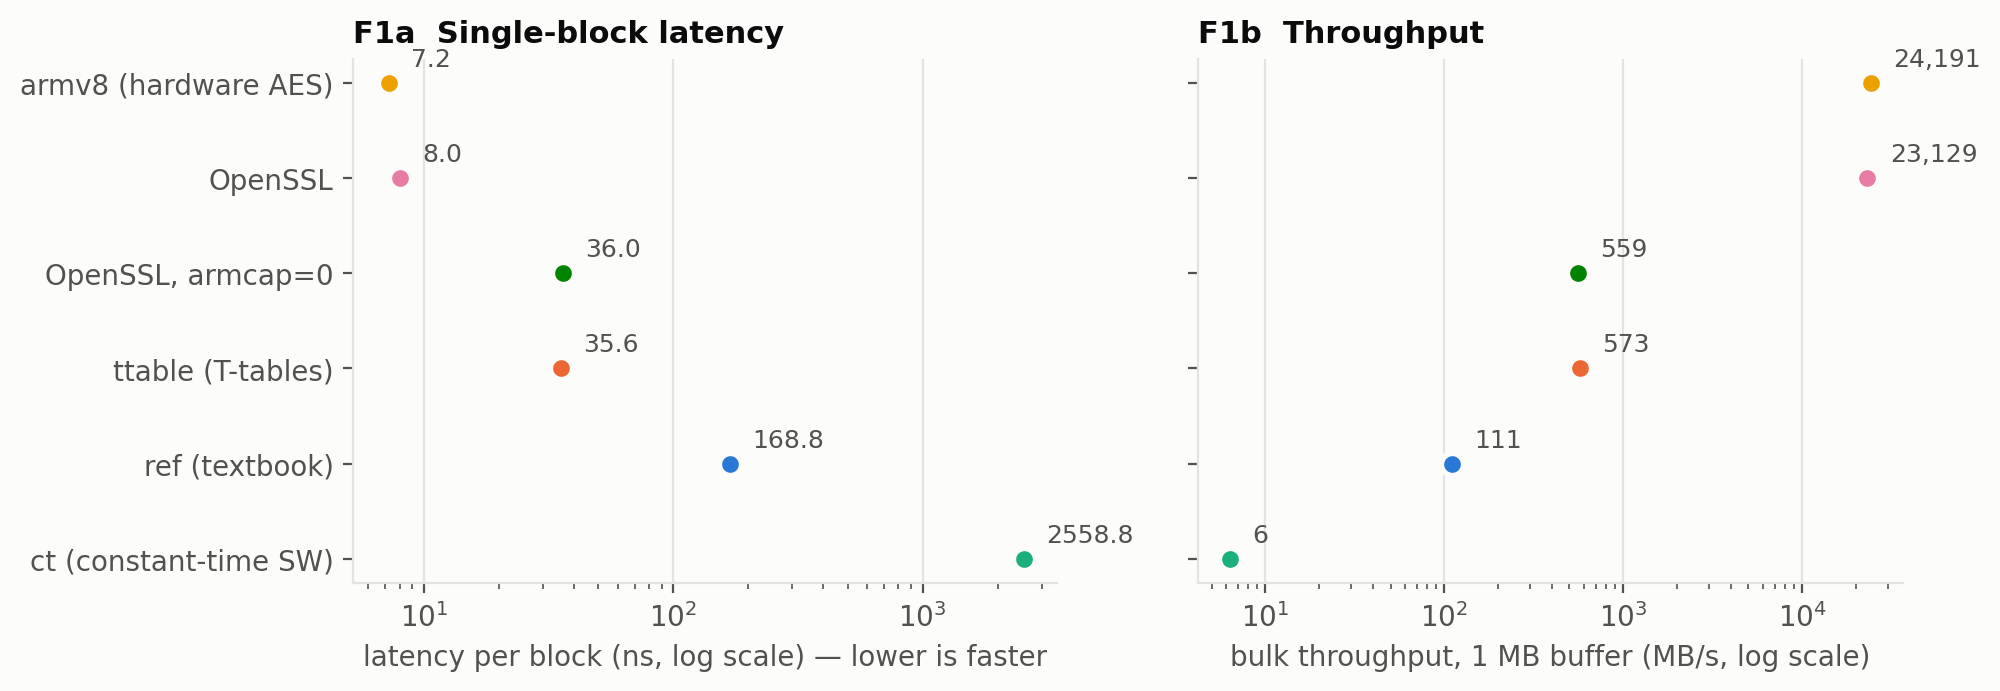
\includegraphics[width=\textwidth]{F1_performance.png}
\caption{Latency and throughput (F1).}
\label{fig:f1}
\end{figure}

The hardware instructions are about 353$\times$ faster than the constant-time software, which pays for its safety by computing the S-box with 11 GF(2$^8$) multiplications per byte. Bit-sliced and vector-permute designs~\cite{kasper09,hamburg09} reduce this gap; the implementation here was written for clarity.

\subsection{Leakage}

\begin{table}[htbp]
\centering
\footnotesize
\renewcommand{\arraystretch}{1.15}
\setlength{\tabcolsep}{3.4pt}
\begin{tabular}{@{}llrrrrrrl@{}}
\toprule
Experiment & Cache & $B$ & $\lvert t\rvert$ & Fixed ns & Random ns & $\Delta$ ns & Min.\ det.\ ns & Verdict \\
\midrule
\textbf{pos\_leaky} (positive) & hot & 94 & \textbf{654.98} & 30.34 & 16.58 & +13.77 & 0.095 & leak \\
aa\_control (negative) & hot & 94 & 1.02 & 16.56 & 16.53 & +0.03 & 0.128 & none \\
pos\_twin (branch-free) & hot & 93 & 4.53 & 31.12 & 31.47 & $-$0.35 & 0.343 & flagged$^\dagger$ \\
ref & hot & 19 & 0.04 & 146.87 & 146.87 & $-$0.00 & 0.283 & none \\
ref & evicted & 1 & 0.06 & 195.80 & 195.78 & +0.02 & 1.59 & none \\
ttable & hot & 95 & 0.48 & 28.57 & 28.66 & $-$0.09 & 0.790 & none$^\dagger$ \\
\textbf{ttable} & \textbf{evicted} & 1 & \textbf{18.79} & 84.10 & 80.97 & \textbf{+3.13} & 0.751 & \textbf{leak} \\
ct & hot & 1 & 0.85 & 2638.40 & 2640.26 & $-$1.86 & 9.82 & none \\
ct & evicted & 1 & 1.05 & 2717.91 & 2664.97 & +52.95 & 227.5 & none \\
armv8 & hot & 2286 & 0.55 & 1.229 & 1.228 & +0.001 & 0.006 & none \\
armv8 & evicted & 1 & 1.10 & 36.20 & 41.72 & $-$5.51 & 22.6 & none \\
openssl & hot & 409 & 1.19 & 6.97 & 6.98 & $-$0.02 & 0.056 & none \\
openssl & evicted & 1 & 1.79 & 40.15 & 40.53 & $-$0.39 & 0.981 & none \\
\textbf{openssl, armcap=0} & hot & 78 & \textbf{19.83} & 33.77 & 34.17 & $-$0.40 & 0.091 & leak$^\dagger$ \\
openssl, armcap=0 & evicted & 1 & 4.44 & 79.58 & 78.16 & +1.43 & 1.45 & borderline \\
\bottomrule
\end{tabular}
\caption{Leakage tests ($N = 10^6$ samples each). $^\dagger$Hot-cache results for code with data-dependent loads: see Section~\ref{sec:unexpected}.}
\label{tab:leak}
\end{table}

\begin{figure}[htbp]
\centering
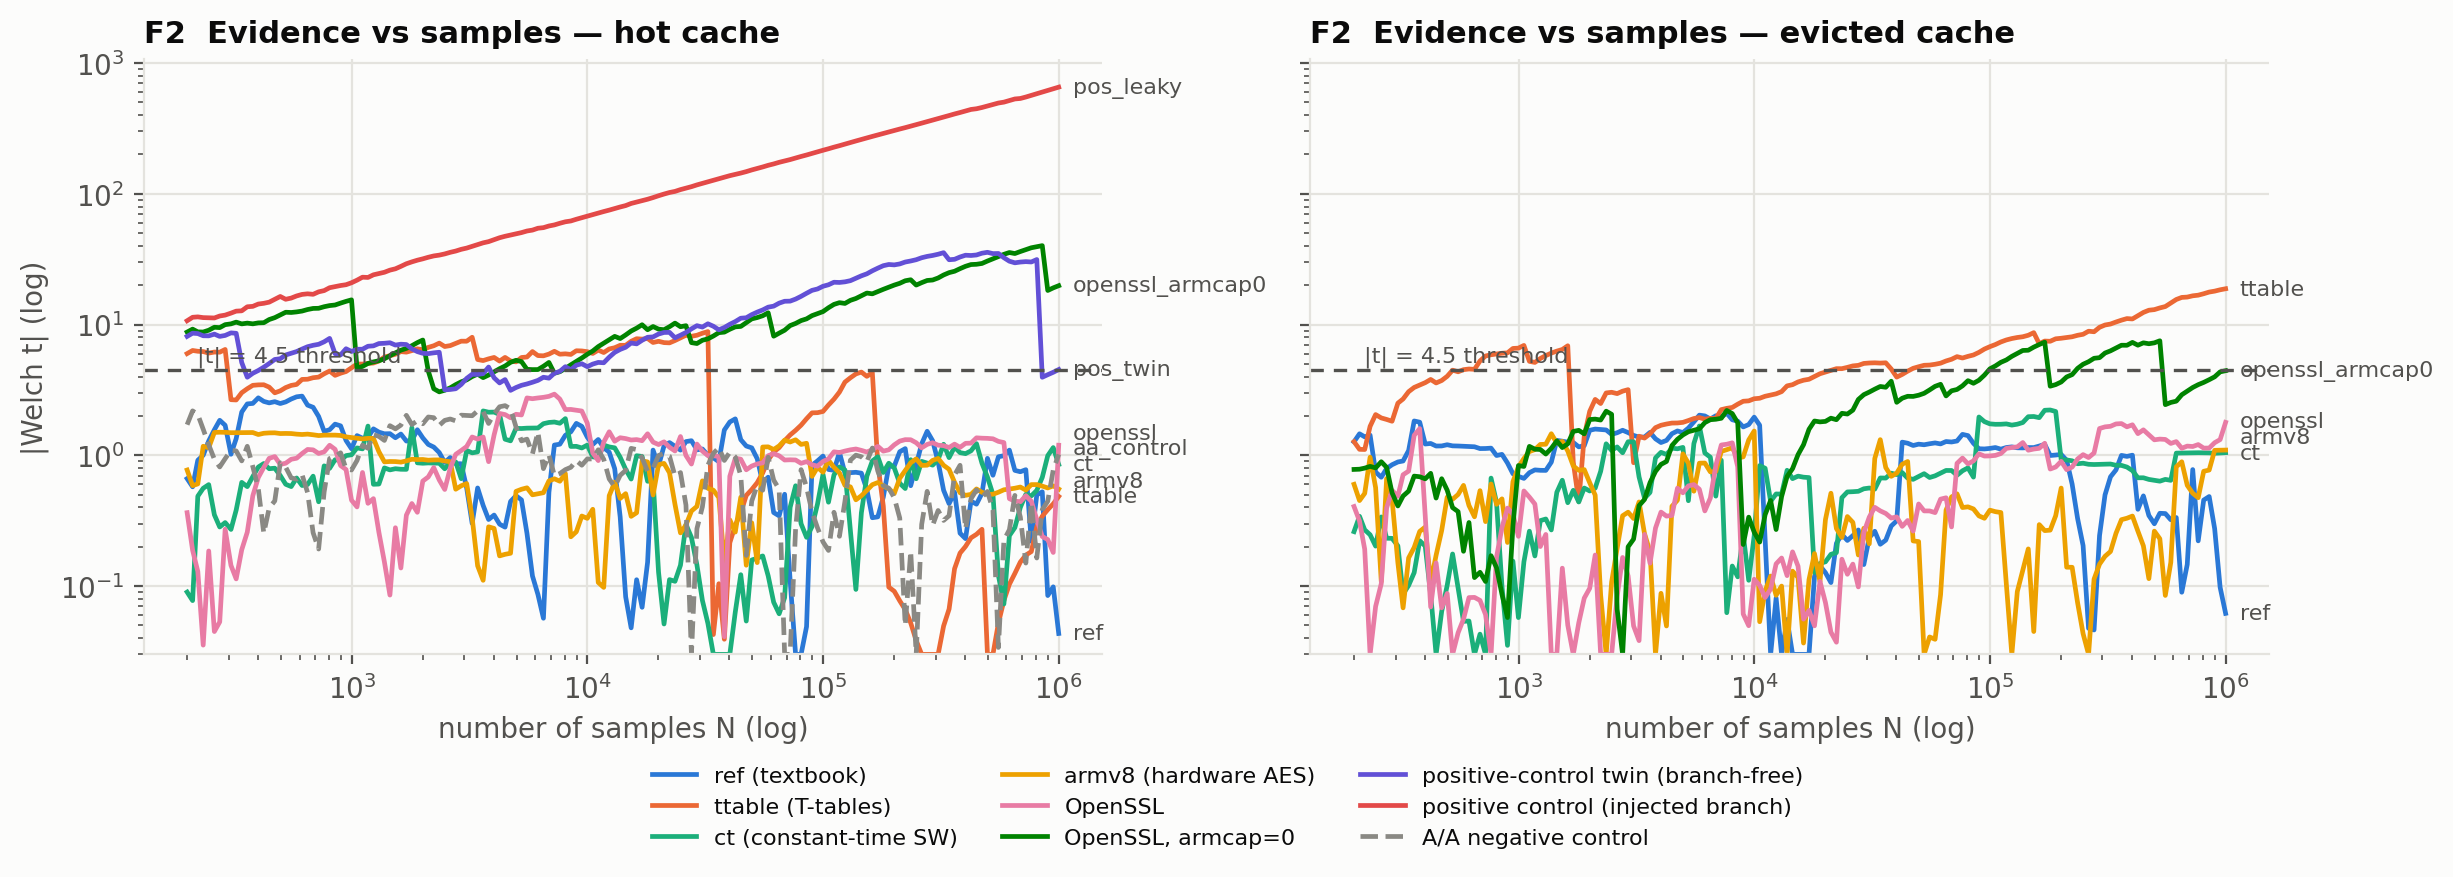
\includegraphics[width=\textwidth]{F2_t_vs_n.png}
\caption{$\lvert t\rvert$ versus number of samples, hot and evicted cache (F2).}
\label{fig:f2}
\end{figure}

Figure~\ref{fig:f2} shows how the evidence accumulates. For a genuine leak, $\lvert t\rvert$ grows roughly as $\sqrt N$, so the positive control rises in a straight line on log--log axes. With no leak, it wanders below the threshold. T-table under eviction keeps rising and stays above 4.5 from $N \approx 4.5\times10^4$.

\begin{figure}[htbp]
\centering
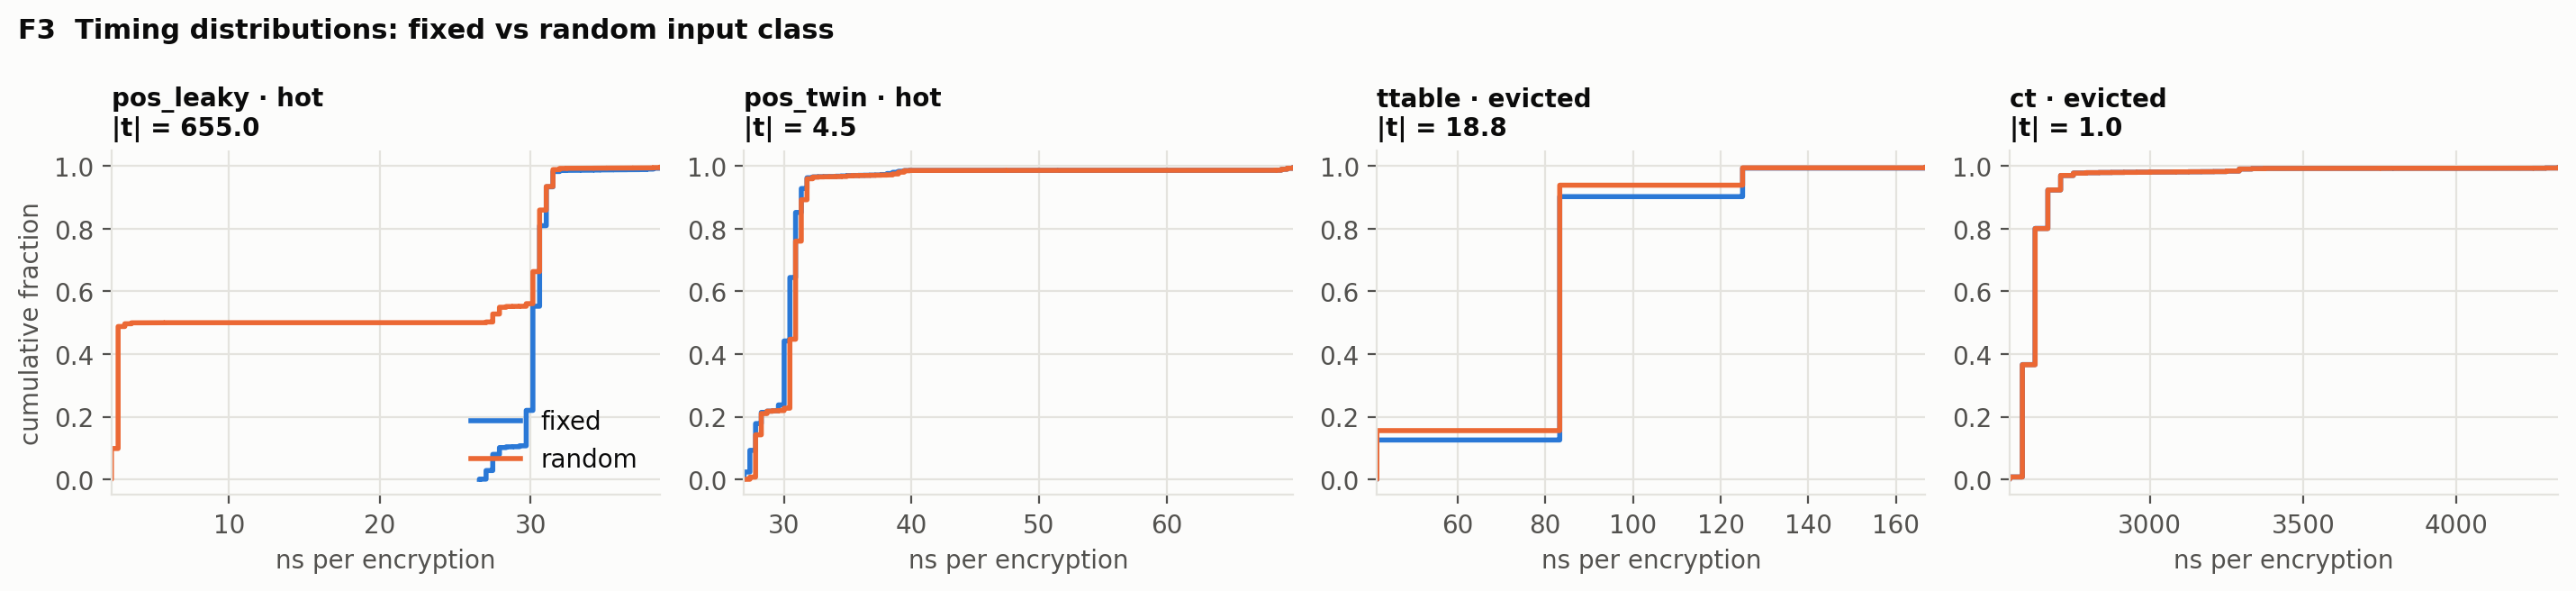
\includegraphics[width=\textwidth]{F3_ecdf.png}
\caption{Timing distributions of the fixed and random classes (F3).}
\label{fig:f3}
\end{figure}

\subsection{Hypothesis verdicts}

\begin{table}[htbp]
\centering
\small
\renewcommand{\arraystretch}{1.15}
\begin{tabular}{@{}P{0.07\textwidth}P{0.16\textwidth}P{0.67\textwidth}@{}}
\toprule
ID & Verdict & Key evidence \\
\midrule
H0 & \tick{} supported & A/A $\lvert t\rvert = 1.02$ (also 0.72 at \code{-O0}) \\
H1 & \tick{} supported & $\lvert t\rvert = 655$; the branch costs 13.8~ns per call on average \\
H2 & \tick{} supported & evicted $\lvert t\rvert = 18.79$, +3.13~ns; Mann--Whitney $p < 10^{-300}$ \\
H3 & \tick{} supported & largest $\lvert t\rvert = 1.10$ across \code{ct} and \code{armv8} in both conditions \\
H4 & \tick{} supported & default $\rightarrow$ \code{aes\_v8\_ecb\_encrypt} at 8.0~ns; \code{armcap=0} $\rightarrow$ \code{AES\_encrypt} at 36.1~ns, flagged \\
\bottomrule
\end{tabular}
\caption{Verdicts on the pre-registered hypotheses.}
\label{tab:verdicts}
\end{table}

\subsection{Compiler behaviour}

\begin{figure}[htbp]
\centering
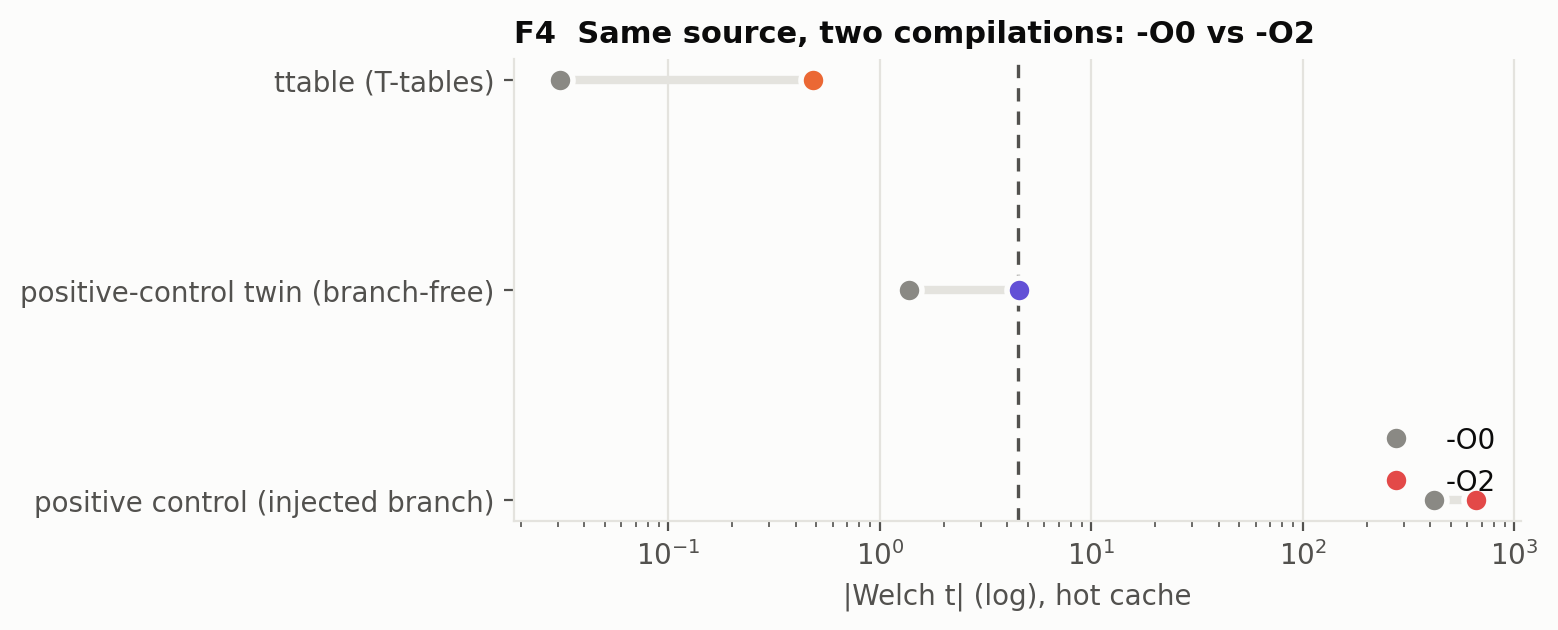
\includegraphics[width=0.85\textwidth]{F4_compiler.png}
\caption{Same source, two compilations: \code{-O0} versus \code{-O2} (F4).}
\label{fig:f4}
\end{figure}

The injected branch survives both compilations and is detected at both: $\lvert t\rvert = 417$ at \code{-O0} and 655 at \code{-O2}. At \code{-O0} the twin is clean ($\lvert t\rvert = 1.38$), while at \code{-O2} it is marginally flagged ($\lvert t\rvert = 4.53$). The \code{-O0} code is about 6$\times$ slower, so the same per-sample effect is diluted.

\subsection{Toy key recovery}

To make ``leakage'' concrete, the attacker side of \code{recover} sees only (plaintext byte, timing) pairs and the public S-box. For each guess $g$ it correlates the mean time per $p_0$ with the predicted pattern $[S(p_0 \oplus g) < \texttt{0x80}]$. Against the injected branch, the secret byte \texttt{0x3C} was ranked first at the first checkpoint (2,500 timings) and stayed first. Against \code{ct}, the true byte finished ranked 77 of 256; across 3 secrets $\times$ 2 seeds its score stayed within $\pm1.05$ standard deviations of the 256 guesses, consistent with noise. \textbf{This is a toy}: the leak exists only because it was injected.

\subsection{Per-byte timing profile}

\begin{figure}[htbp]
\centering
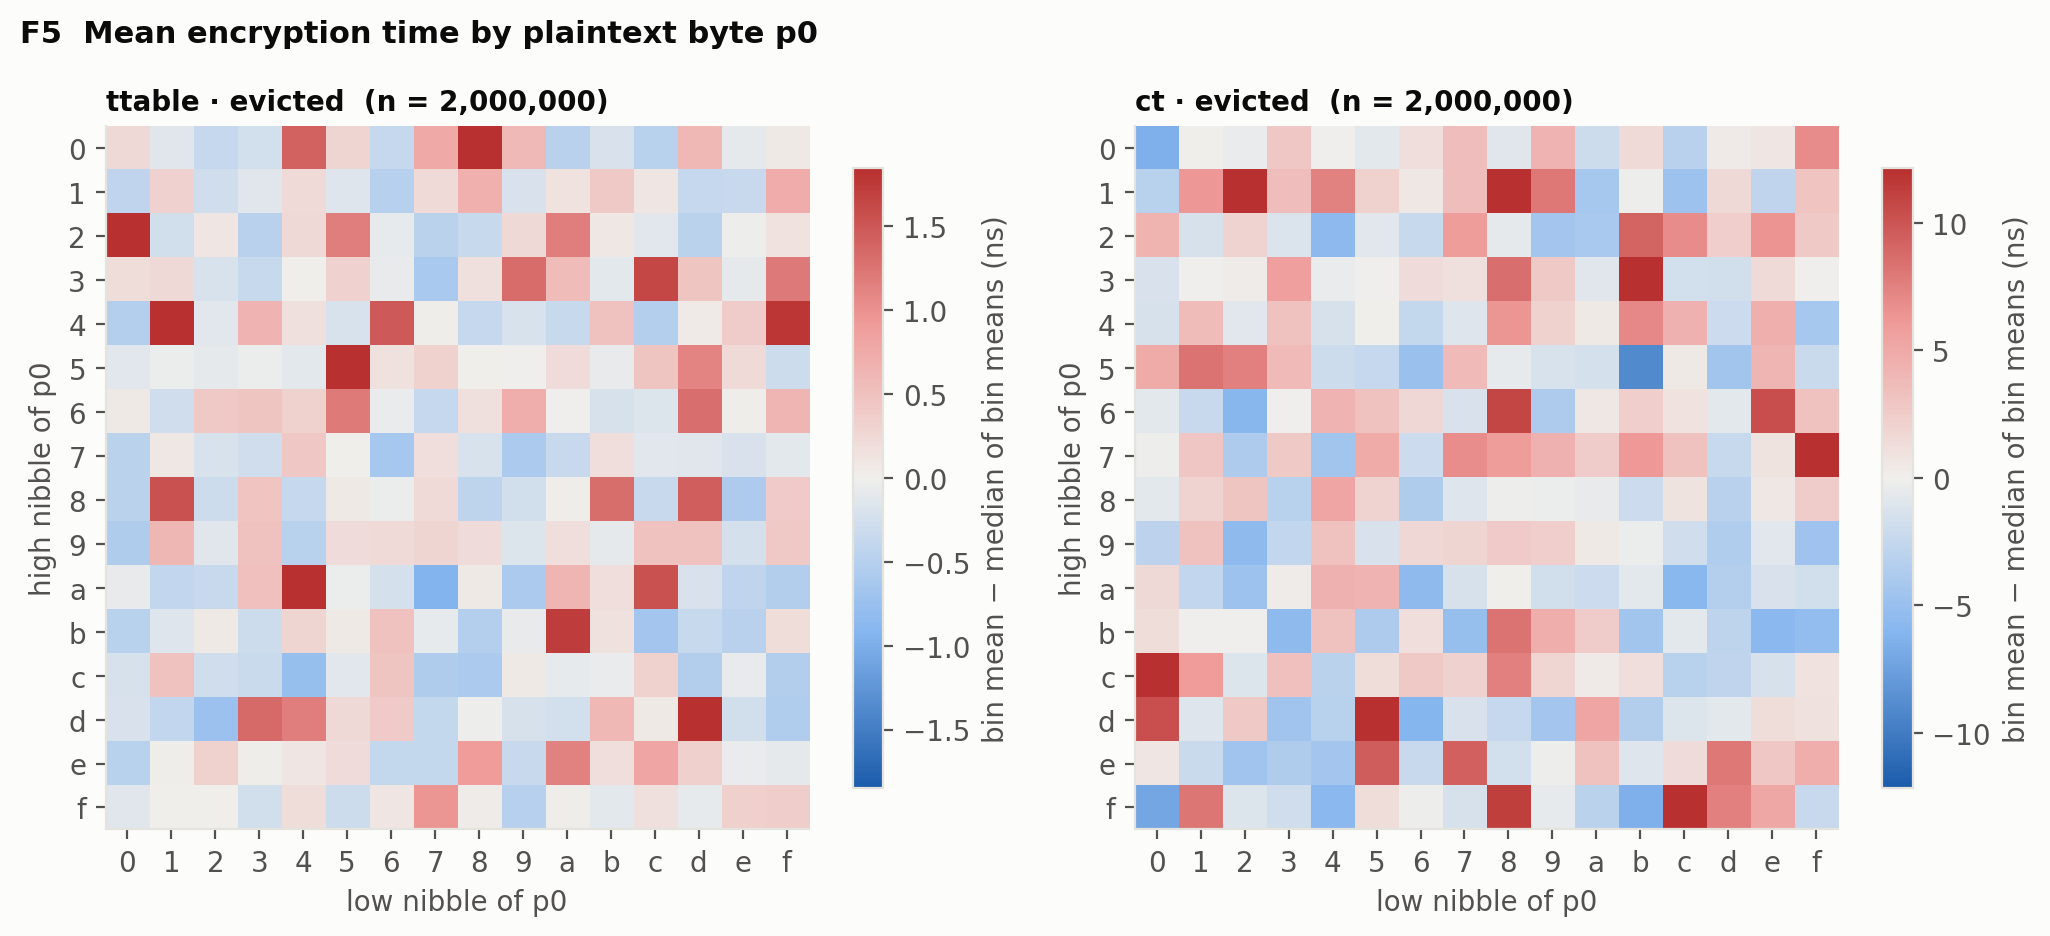
\includegraphics[width=\textwidth]{F5_profile.png}
\caption{Mean encryption time by plaintext byte $p_0$ under eviction, $2\times10^6$ samples (F5).}
\label{fig:f5}
\end{figure}

Even with $2\times10^6$ evicted samples, neither the T-table nor the constant-time profile shows visible structure by $p_0$ (Figure~\ref{fig:f5}). The fixed-versus-random test detects \emph{that} the T-table implementation's timing depends on the data, but locating \emph{which} byte values are slow, as a real cache attack needs~\cite{bernstein05}, would require far more samples or a stronger attacker model such as Prime+Probe~\cite{osvik06}. Detecting a leak is much easier than exploiting it.

\section{Screenshots of the developed system}
\label{sec:screens}

\begin{figure}[htbp]
\centering
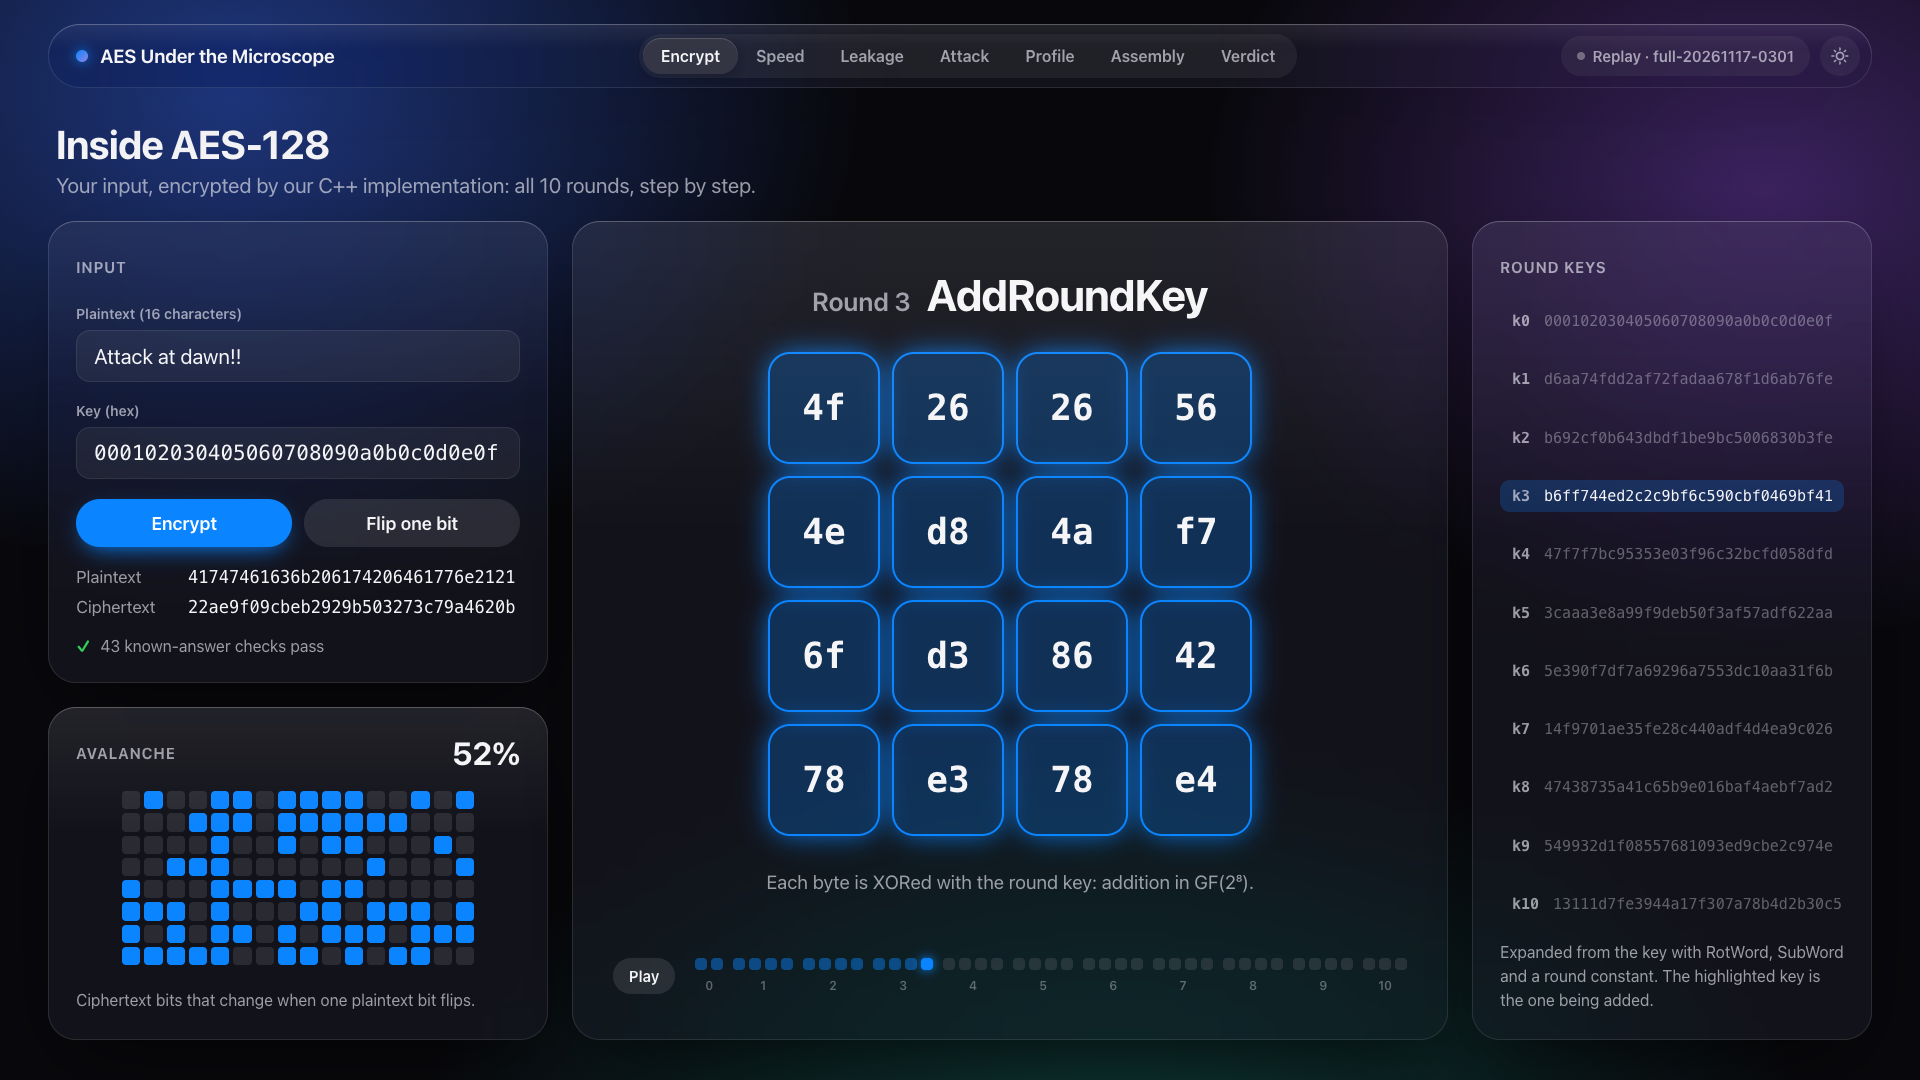
\includegraphics[width=\textwidth]{dash_explorer.png}
\caption{Dashboard, Encrypt view: a user-supplied plaintext encrypted round by round, with round keys and the avalanche effect.}
\label{fig:dash_explorer}
\end{figure}

\begin{figure}[htbp]
\centering
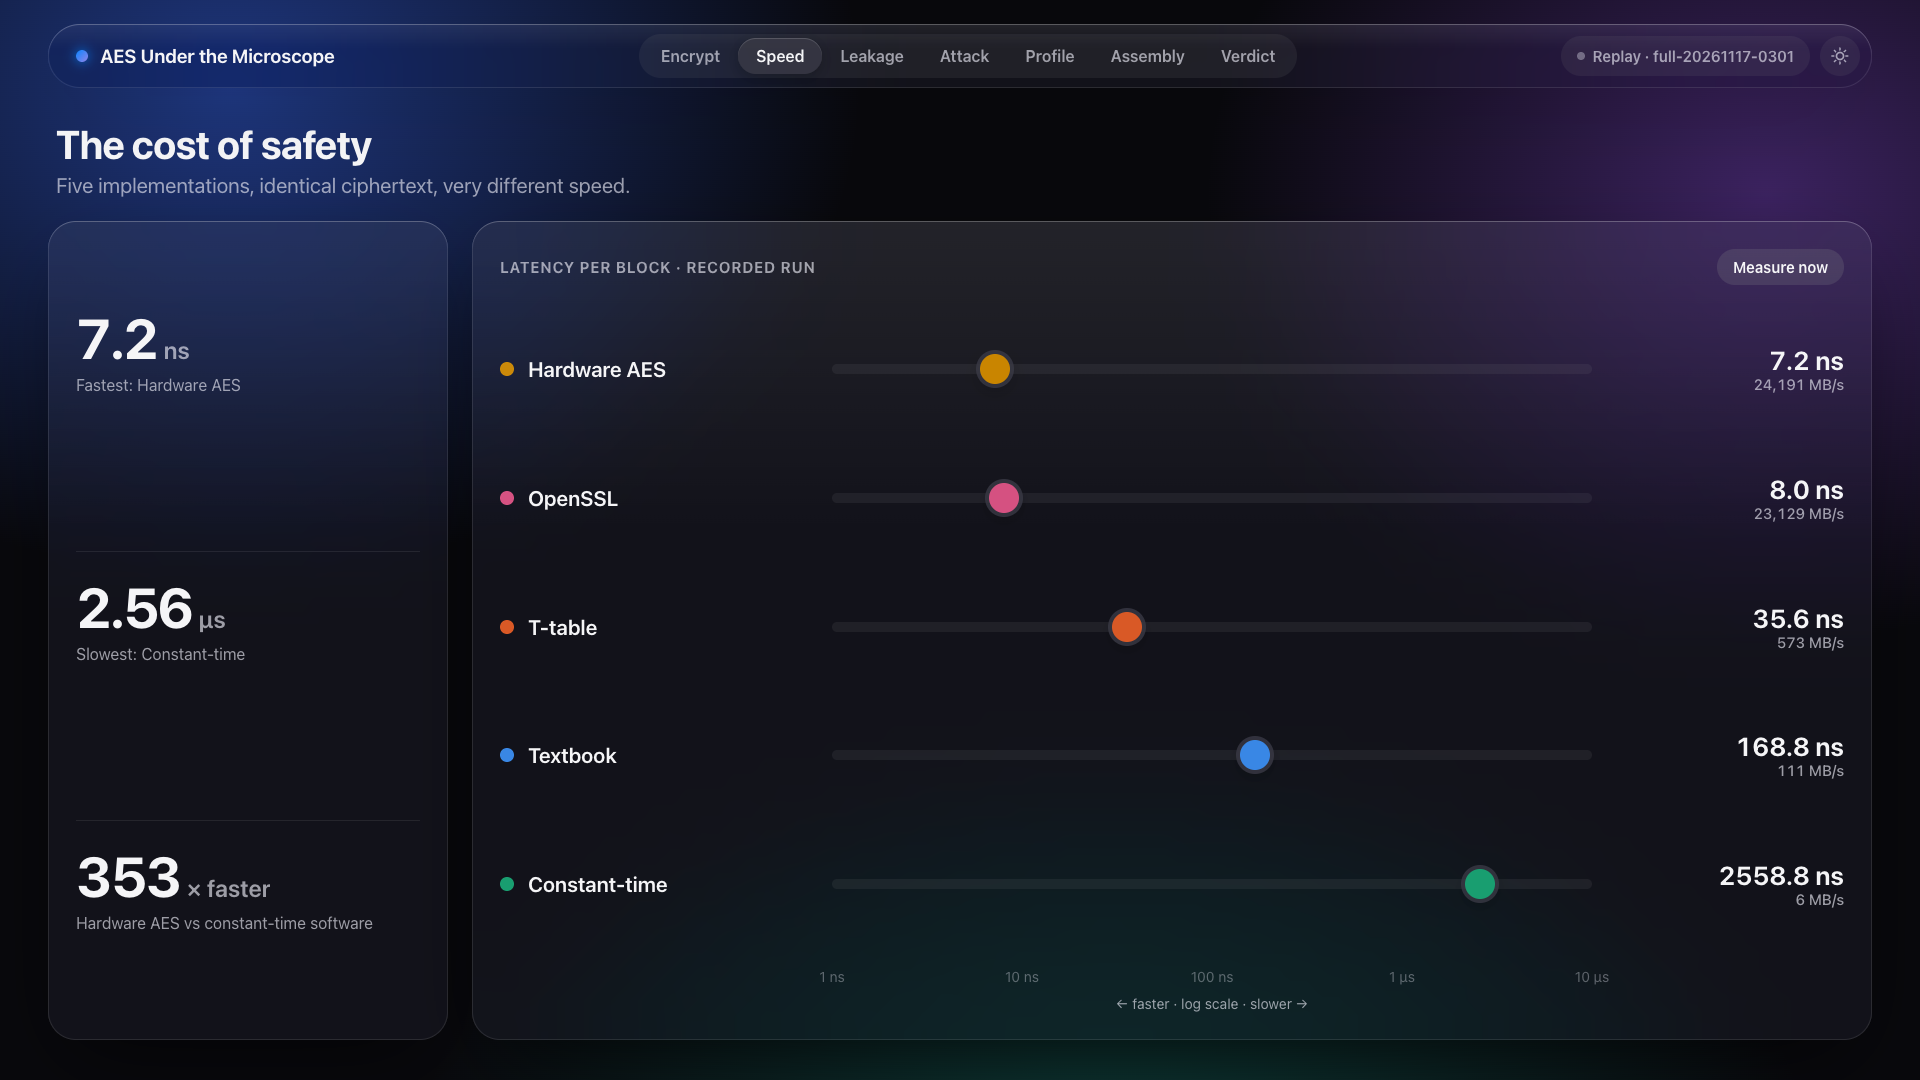
\includegraphics[width=\textwidth]{dash_speed.png}
\caption{Dashboard, Speed view: latency and throughput of the implementations.}
\label{fig:dash_speed}
\end{figure}

\begin{figure}[htbp]
\centering
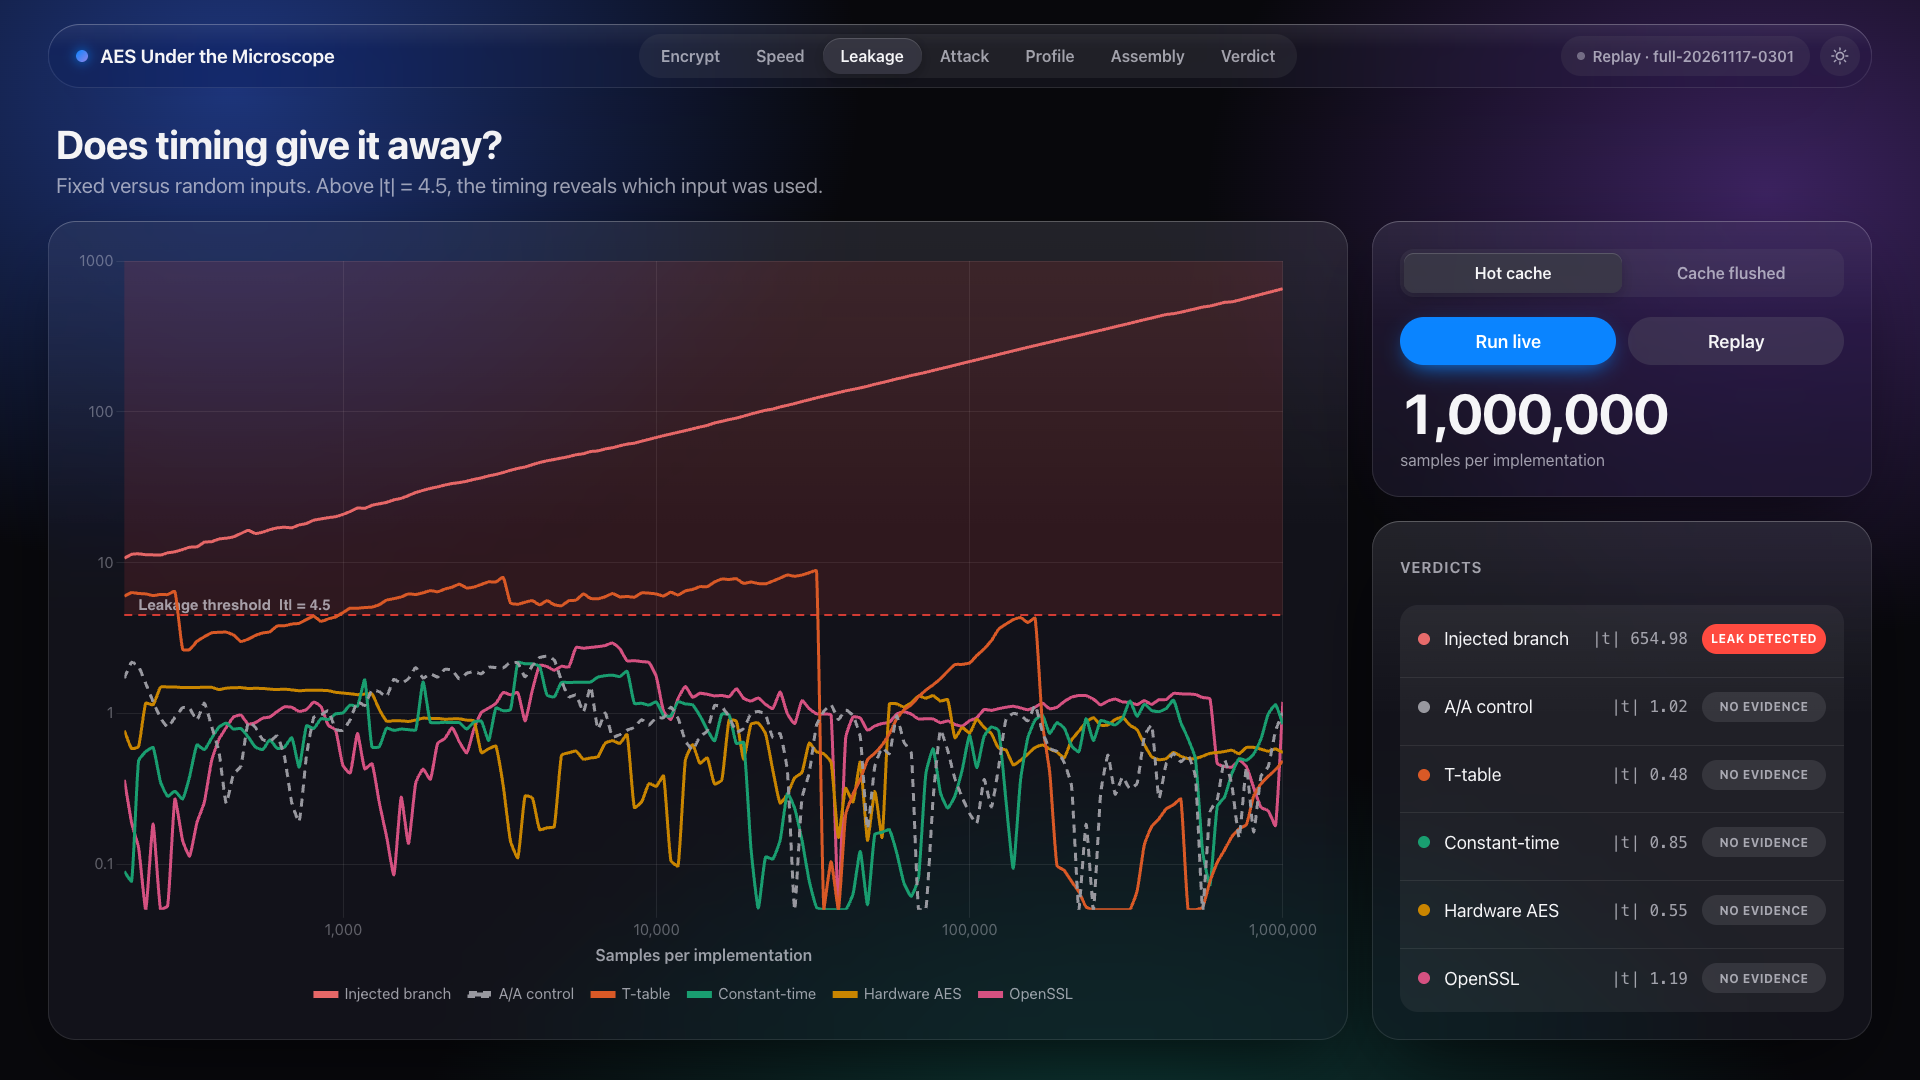
\includegraphics[width=\textwidth]{dash_race.png}
\caption{Dashboard, Leakage view: $\lvert t\rvert$ against samples for all implementations (recorded run, hot cache).}
\label{fig:dash_race}
\end{figure}

\begin{figure}[htbp]
\centering
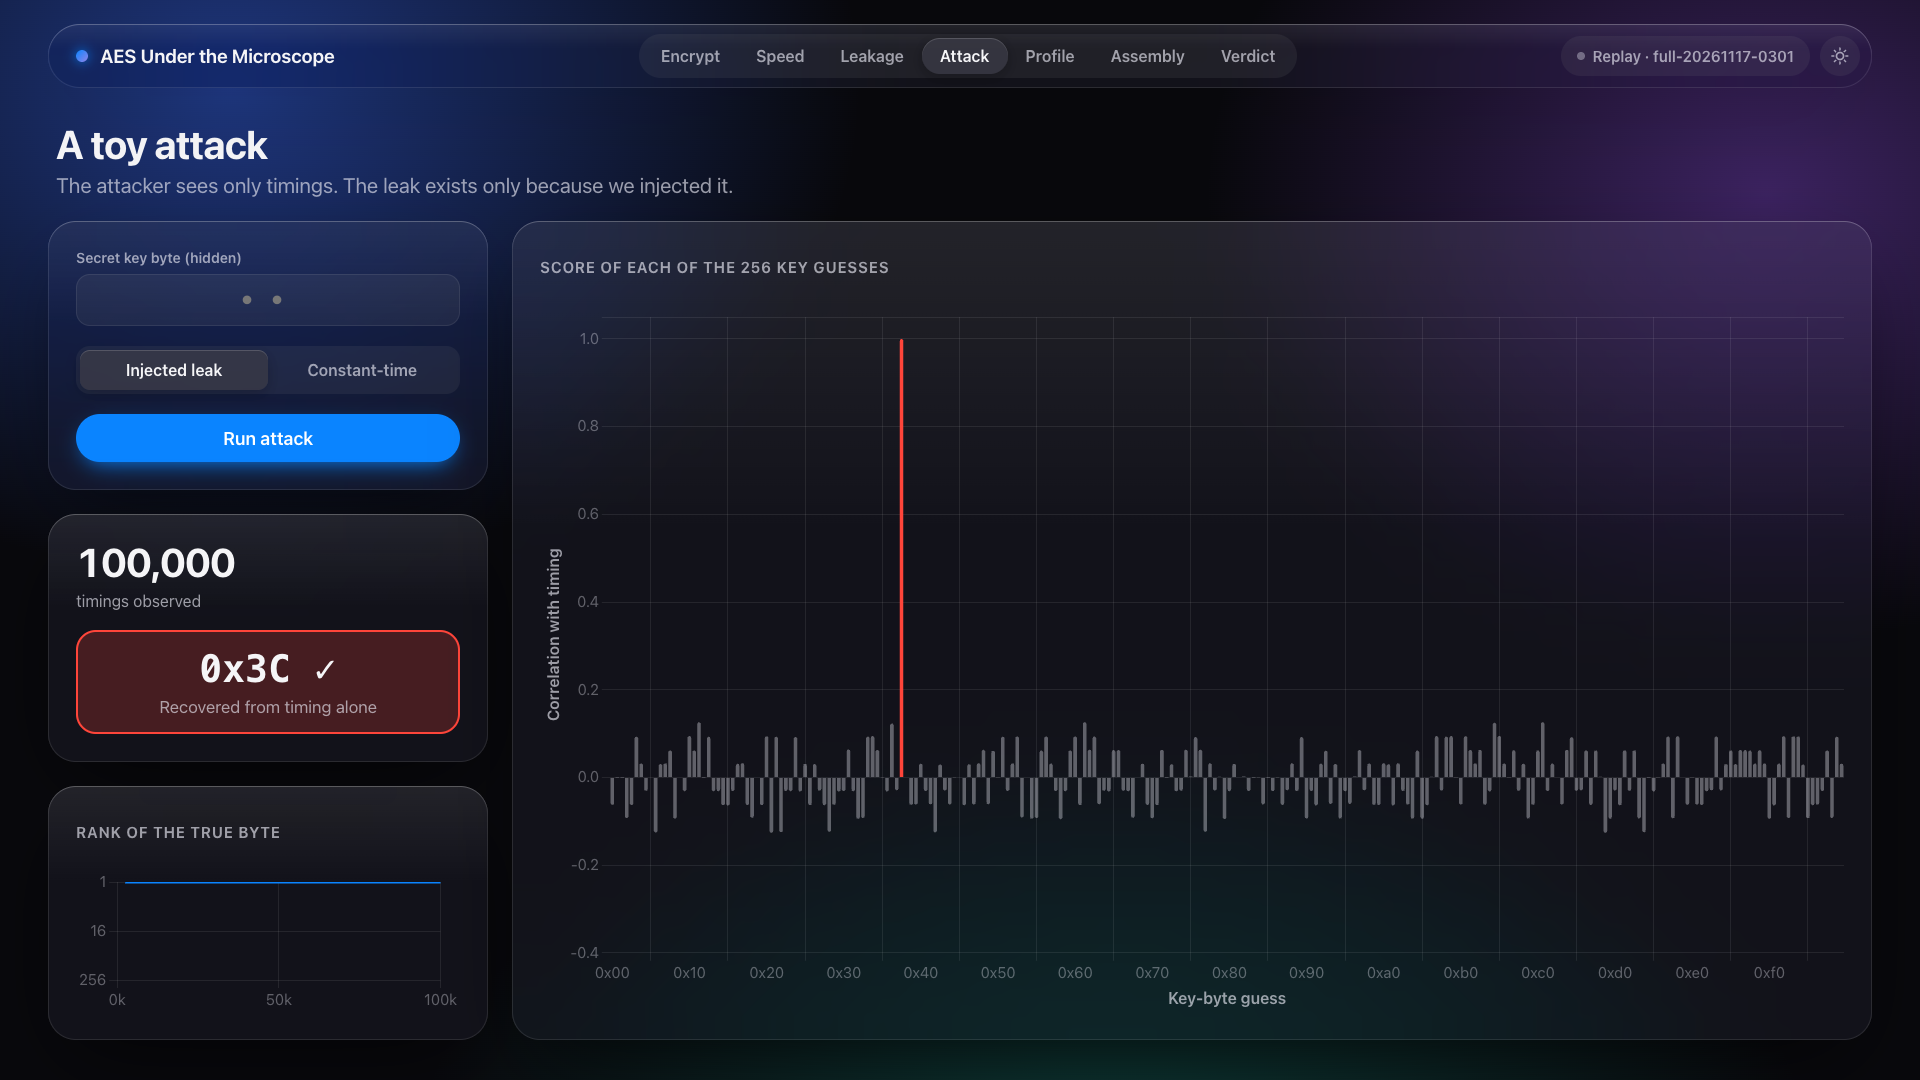
\includegraphics[width=\textwidth]{dash_heist.png}
\caption{Dashboard, Attack view: the secret byte \texttt{0x3C} recovered from timing alone, only against the injected branch.}
\label{fig:dash_heist}
\end{figure}

\begin{figure}[htbp]
\centering
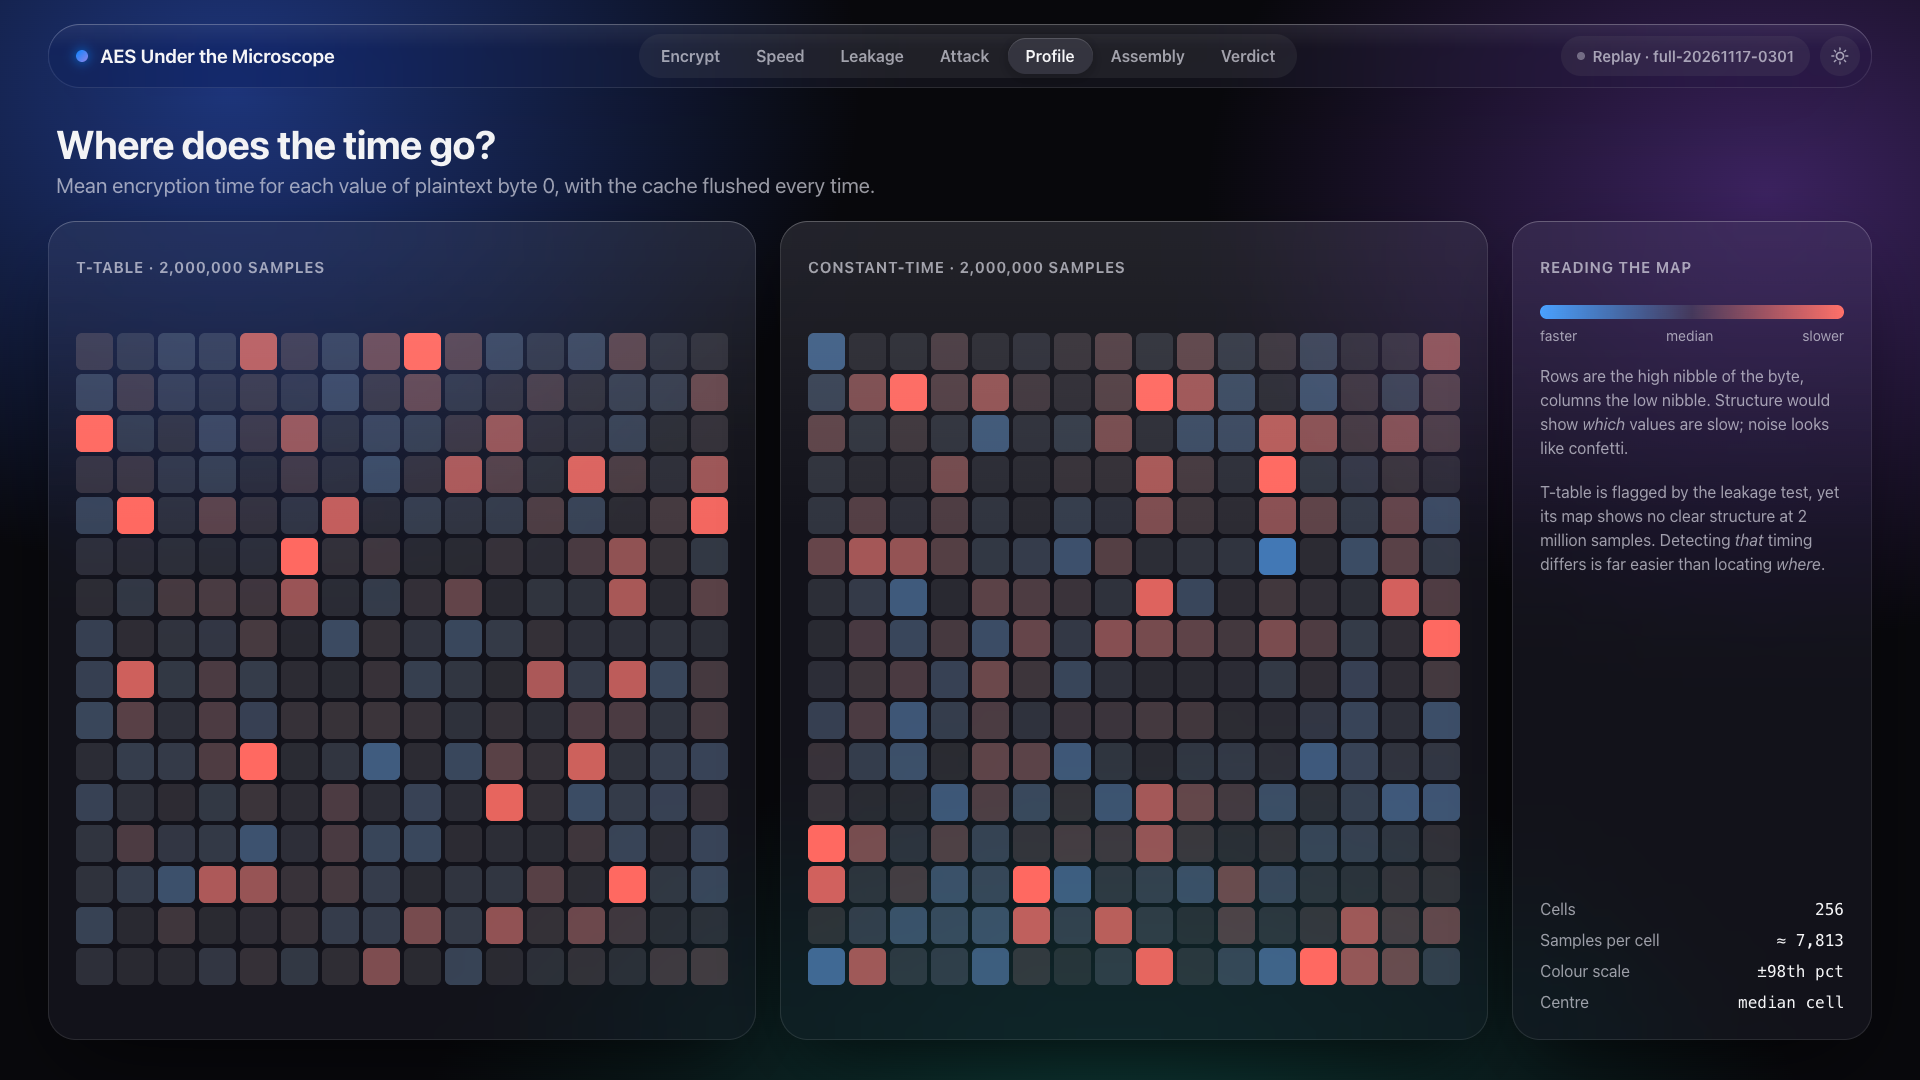
\includegraphics[width=\textwidth]{dash_heatmap.png}
\caption{Dashboard, Profile view: mean time per plaintext byte under eviction, T-table versus constant-time.}
\label{fig:dash_heatmap}
\end{figure}

\begin{figure}[htbp]
\centering
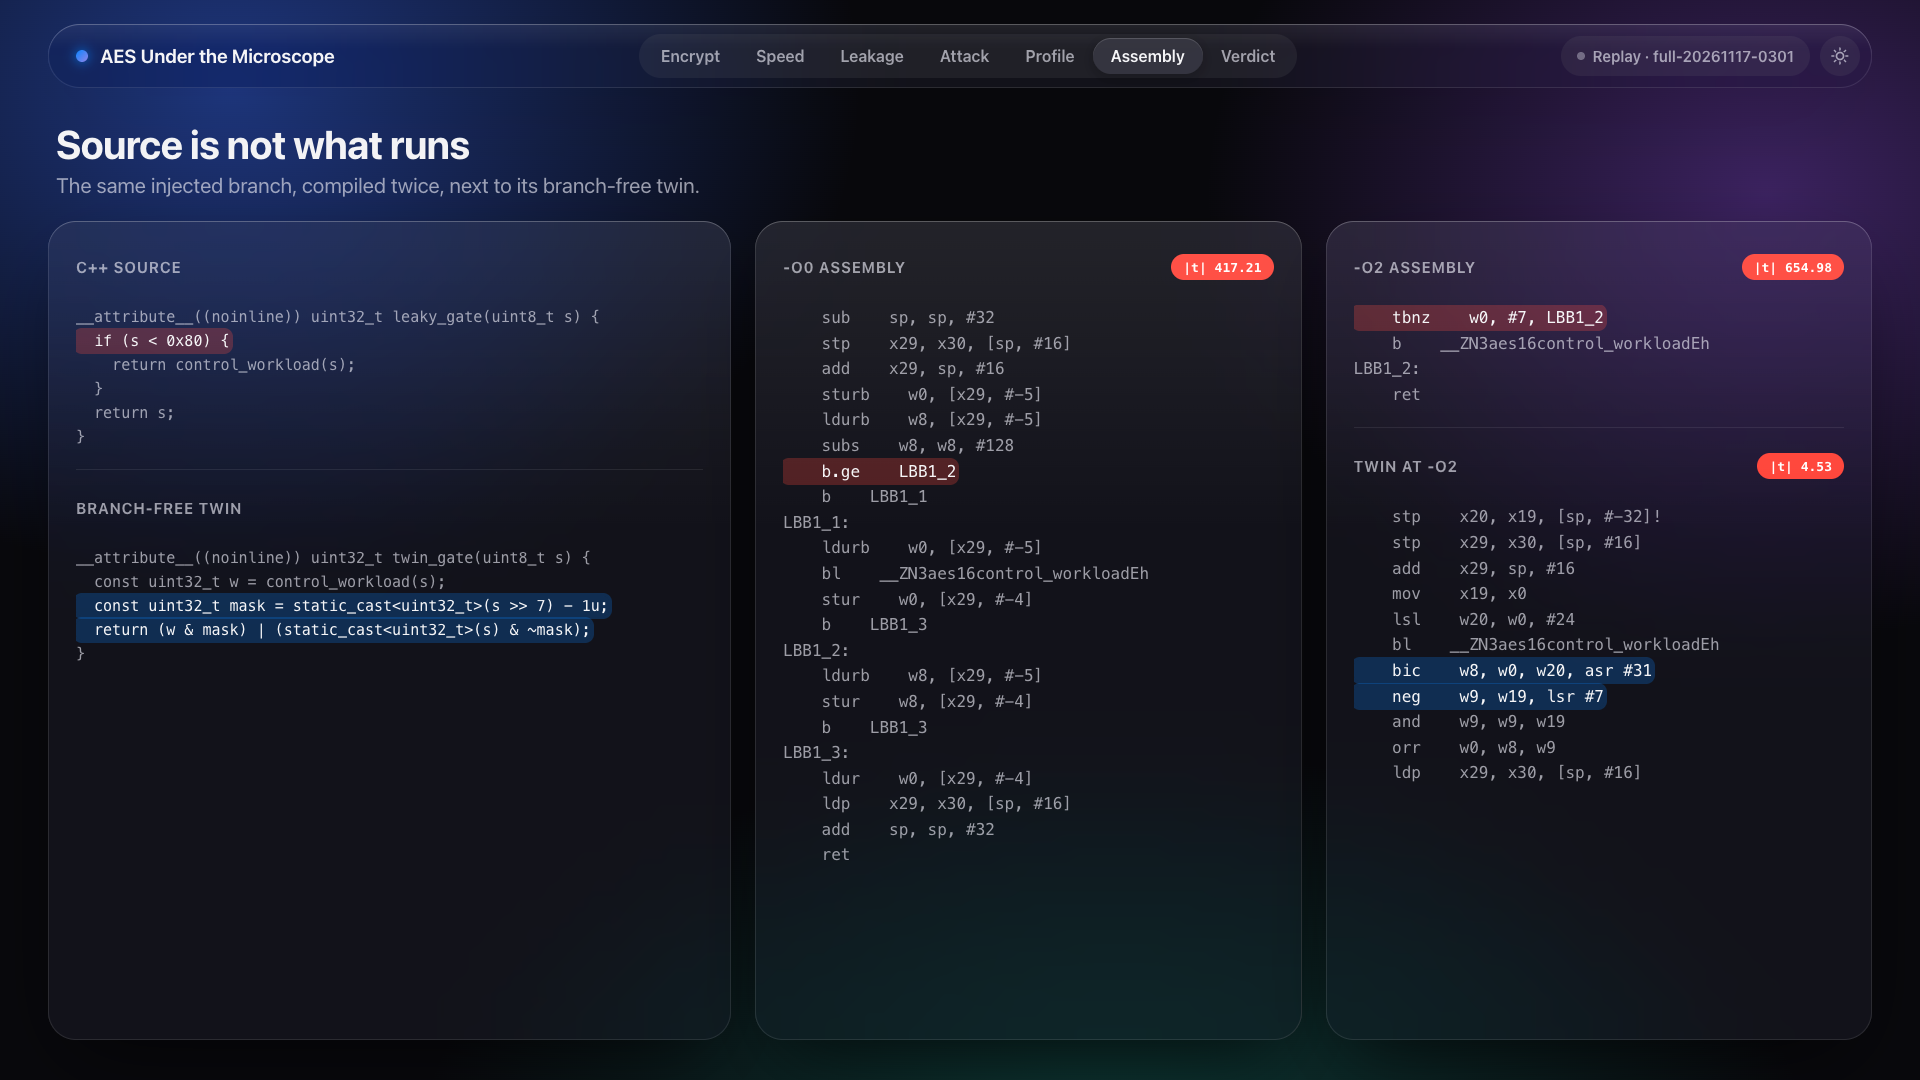
\includegraphics[width=\textwidth]{dash_compiler.png}
\caption{Dashboard, Assembly view: the injected branch survives as \code{tbnz} at \code{-O2}; the twin uses a mask.}
\label{fig:dash_compiler}
\end{figure}

\begin{figure}[htbp]
\centering
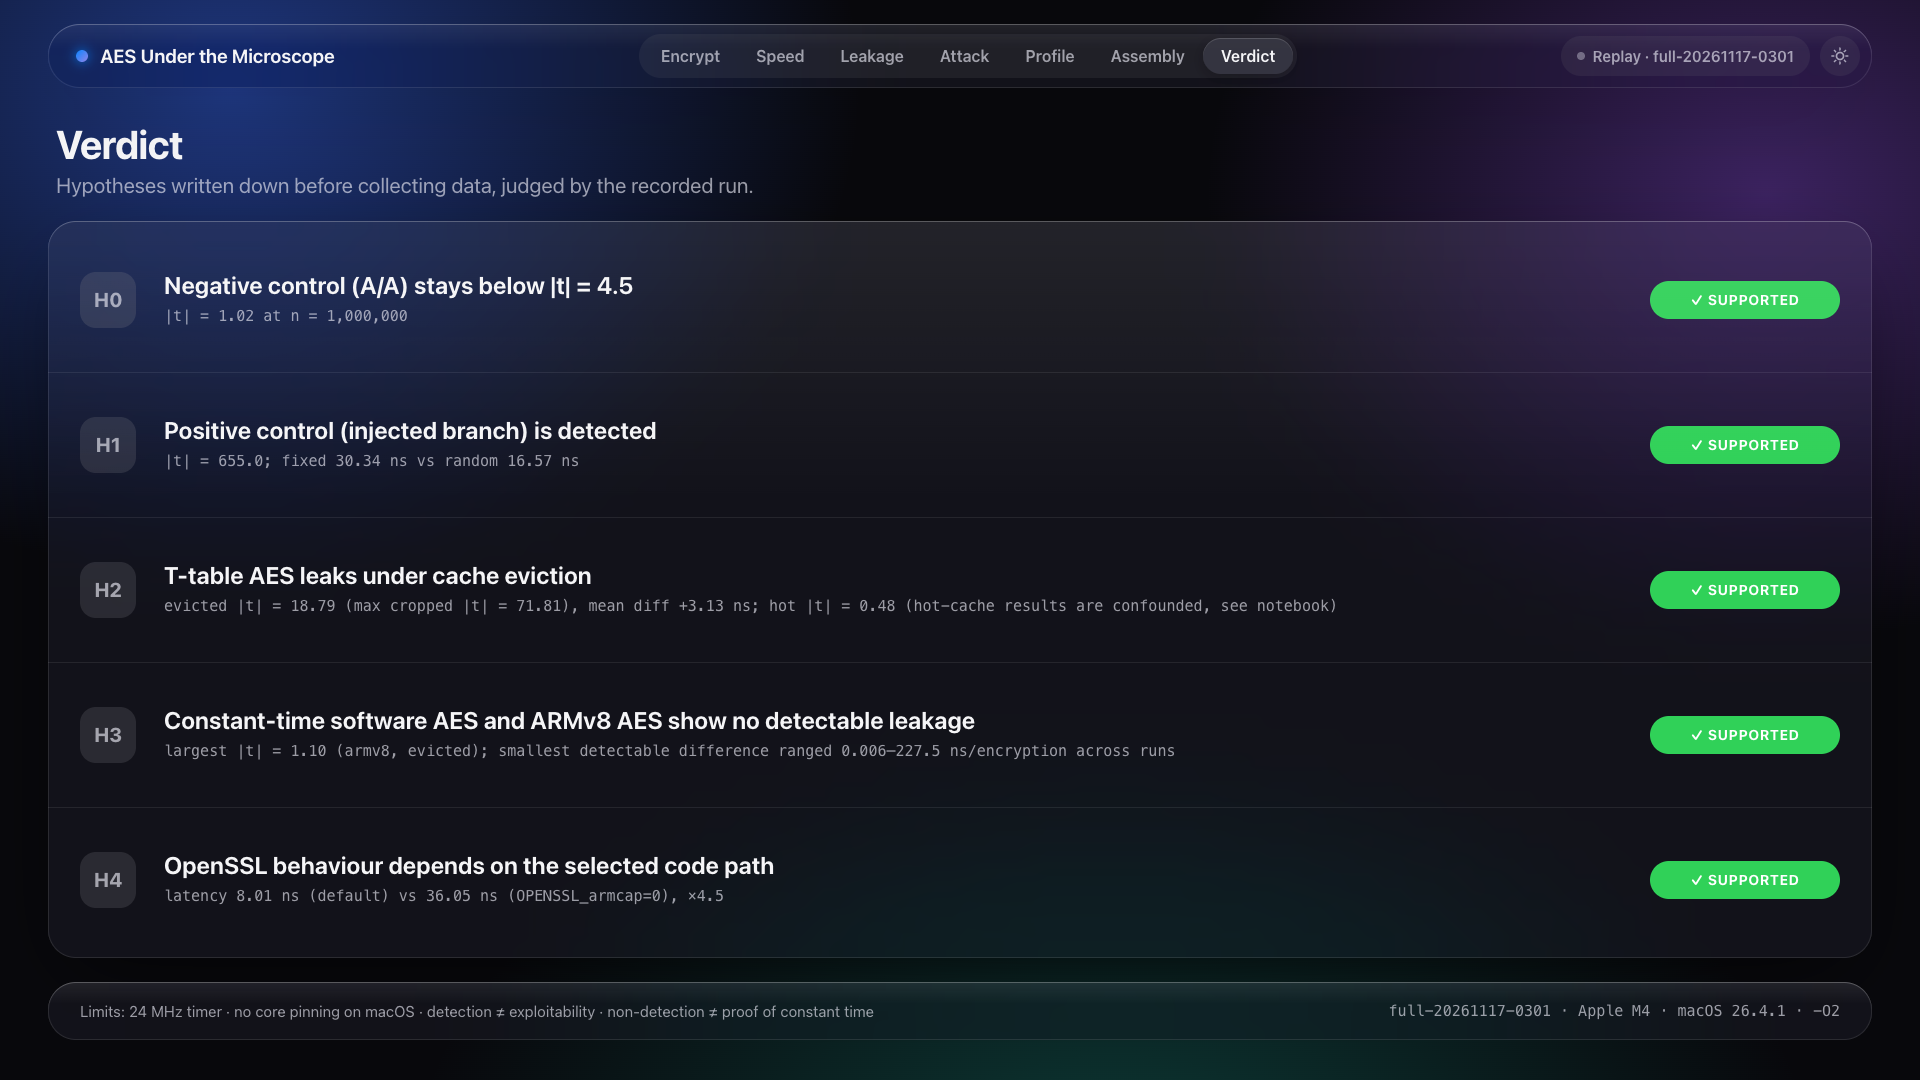
\includegraphics[width=\textwidth]{dash_scorecard.png}
\caption{Dashboard, Verdict view: each pre-registered hypothesis judged against the recorded run.}
\label{fig:dash_scorecard}
\end{figure}

\section{Discussion}

\subsection{What the clean results show}

The cache condition matters, as H2 predicted. In a hot loop, the M4's 128~KB L1D holds all 4~KB of T-tables and the mean timing showed no difference ($\lvert t\rvert = 0.48$). Once the cache is flushed before every encryption, approximating an attacker who evicts the victim's data, the T-table implementation leaks: 3.1~ns per encryption on an 81~ns operation. Interestingly the \emph{fixed} class is slower, the opposite of a simple miss-count model (the all-zero plaintext puts all first-round lookups of a table in one line); the direction is reported as observed, without a confirmed mechanism.

The textbook \code{ref} implementation did not leak, even under eviction. Its 256-byte S-box occupies only two 128-byte lines, so after the first lookup of a block almost every access hits. Small tables leak far less than large ones on a 128-byte-line machine.

\code{ct} and \code{armv8} showed no evidence in either condition, consistent with the assembly. The non-detections are bounded: for \code{armv8} hot, any mean difference above 0.006~ns would have been detected. For the evicted runs the bound is weak (22.6~ns for \code{armv8}, 227.5~ns for \code{ct}), because a single encryption lasts less than one timer tick and eviction adds large variance.

\subsection{An unexpected result: branch-free code flagged in the hot regime}
\label{sec:unexpected}

The branch-free twin was flagged in development runs ($\lvert t\rvert = 6$--15 at $N = 2\times10^5$) and marginally in the final run ($\lvert t\rvert = 4.53$ at $10^6$). The investigation was time-boxed and recorded in the lab notebook (Table~\ref{tab:investigation}).

\begin{table}[htbp]
\centering
\small
\renewcommand{\arraystretch}{1.15}
\begin{tabular}{@{}P{0.55\textwidth}P{0.35\textwidth}@{}}
\toprule
Hypothesis or check & Outcome \\
\midrule
Assembly: is the twin really branch-free? & Yes \\
Input-preparation path differs between classes & Fixed; effect persisted \\
Choice of fixed plaintext & Four choices, all flagged \\
Each component in isolation (workload, gate, S-box load), DIT on and off & No effect \\
Loaded address vs.\ loaded value, separated & No effect in isolation \\
Dependence on batch size & Present only for $B \ge 94$, absent at $B \le 10$ \\
Hardware AES on its own & Never shows it \\
\bottomrule
\end{tabular}
\caption{Investigation of the hot-regime effect.}
\label{tab:investigation}
\end{table}

A plausible but \textbf{unconfirmed} explanation is microarchitectural state that persists across samples: the fixed class repeats identical inputs and can benefit from predictors trained on earlier fixed samples, such as the load-address and load-value predictors reported on recent Apple cores~\cite{flop,slap}; the random class cannot. Consequently, on this platform hot-cache, long-batch detections of code with data-dependent loads cannot be attributed to cache leakage on their own, which is why the OpenSSL fallback's hot result is marked. The cache conclusions rest on the evicted runs ($B = 1$), where the effect was absent.

\subsection{Source, machine code, runtime}

\begin{itemize}
  \item \textbf{Source to machine code.} The \code{if} stayed a branch at both \code{-O0} and \code{-O2}. Clang rewrote one multiplication in \code{ct} into shift-and-subtract but kept it branch-free.
  \item \textbf{Machine code to runtime.} Code with no secret branch and no secret-indexed load still produced fixed-versus-random differences under specific conditions.
  \item \textbf{Runtime to statistics.} A significant $\lvert t\rvert$ depends on the cache condition, the batch size and the statistic chosen.
\end{itemize}

\subsection{OpenSSL}

Debugger breakpoints confirmed that by default OpenSSL runs \code{aes\_v8\_ecb\_encrypt}, i.e.\ the AES instructions. With \code{OPENSSL\_armcap=0} it skips both the hardware and the vector-permute code and runs the portable C \code{AES\_encrypt}, whose speed (36~ns) matches the T-table implementation. The default configuration on this machine is therefore the safe one; silently disabling capability detection (for example under emulation) would change both performance and leakage.

\section{Assembly observations}

\begin{itemize}
  \item \code{ref}: 32 \code{ldrb w, [x\_sbox, x\_index]} loads where the index is a state byte; \code{ttable}: 32 \code{ldr w, [x\_table, w\_index, uxtw \#2]} loads. These are the secret-dependent addresses.
  \item \code{ct}: the parallel S-box is 917 straight-line instructions with 0 branches and 0 indexed loads. A remaining assumption is that \code{mul} has data-independent latency, which Apple ties to the DIT bit.
  \item \code{armv8}: 60 \code{aese} and 54 \code{aesmc} instructions.
  \item Positive control: \code{tbnz w0, \#7} at \code{-O2} and \code{subs w8, w8, \#128; b.ge} at \code{-O0}; the twin uses \code{bic}/\code{neg}/\code{and}/\code{orr}, a mask-based select.
  \item OpenSSL: \code{libcrypto.3.dylib} contains 4,190 \code{aese} instructions and four AES families (\code{aes\_v8\_*}, \code{vpaes\_*}, \code{bsaes\_*} and the C \code{AES\_encrypt}).
\end{itemize}

\section{Limitations}

\begin{itemize}
  \item \textbf{Timer:} 41.67~ns resolution; single-encryption evicted samples are heavily quantised, giving weak bounds on non-detection.
  \item \textbf{No cycle counters:} Apple Silicon's cycle counters need private frameworks and root.
  \item \textbf{Scheduling:} no core pinning on macOS, only a QoS hint.
  \item \textbf{One machine, one OS build, one compiler.}
  \item \textbf{Attacker model:} in-process, idealised whole-cache eviction; no cross-process or remote attack.
  \item \textbf{Hot-regime effect:} unexplained (Section~\ref{sec:unexpected}).
  \item \textbf{Single fixed plaintext and key} per test.
  \item \textbf{Live dashboard runs are illustrative only}; reported numbers come from the recorded run.
\end{itemize}

\section{Security implications}

\begin{enumerate}
  \item Table-based AES should not protect secrets on systems where an attacker can influence the cache. Even on a large-L1 machine, eviction made the leak visible within about $4.5\times10^4$ measurements.
  \item Use the hardware instructions, or a vetted library that uses them, and verify that the hardware path is actually selected: OpenSSL's fallback is table-based.
  \item ``Constant-time'' is a property of machine code on a specific CPU, not of source code. Inspect the assembly, then test empirically with controls, and interpret results against a stated sensitivity.
  \item Statistical leakage tests need controls. Without the A/A control the harness could not be shown to be calibrated; without the positive control it could not be shown to detect anything; without the branch-free twin the confound in Section~\ref{sec:unexpected} would have been missed.
\end{enumerate}

These conclusions lead directly to Part II: if constant-time behaviour is decided by the compiler and the processor, the next question is how reliably a language's constant-time mechanisms survive compilation.
